\chapter{开放城市系统}

城市的组织是复杂的。我们经常用模糊场所来描述不同空间区域在城市中所承担的分工。而一个空间位置也可能同时从属于不同的场所。城市科学的研究对象与生态系统有着类似的性质。在生态系统中,多个组分相互作用导致各自在系统中的种群密度发生变化。在城市中,市民对居住条件、工作条件的要求,企业对物流链、地租、工作环境的要求,也使得城市区域分化成了有一定特征的模式。在\cite{christopherson1986city}中提到了一种观点,称城市为一个工作站。这是因为城市是一个集合了各种工具,并由于其中复杂的相互依存、相互促进的关系而演化形成的生产单元。

这些复杂的城市元素在空间上的交互关系经过一定程度上的抽象,可以理解为城市功能在空间上涌现、迁移、或消失而组成的过程。这个过程与人类移动性\cite{molas2017field,gonzalez2008understanding,song2010limits,song2010modelling}的研究有一定的不同。城市功能的功能更具有确定性,空间特征更加明显。同时也更不可逆,是不同于基本的元人口生成模型的,也有必要单独进行建模研究。举例来说,根据\cite{banerjee2015competitive},城市标度律的形成并不一定是简单的规模效应的产物,也有可能是多方博弈的结果。以犯罪的超线性为例:默认的假设是,犯罪的超线性扩展与其他城市属性一样,是由于规模效应而产生的(也就是说,犯罪分子之间更多的联系会增加犯罪的收益)。但是,我们通常忽略的一个事实是,犯罪的发起与城市人口呈线性关系,执法人员的数量与城市人口亦呈线性关系。在\cite{banerjee2015competitive}的模型中,犯罪与执法的博弈机制成功复现了上面的标度律机制。并且该模型亦能解决某些特定类型犯罪的线性标度行为。可见,基于微观元素交互的空间模型有着比依附型生成模型更加丰富的内涵。

我们将城市考虑为生态系统的时候,城市间的流就是绕不开的问题。不同城市之间有着不同的产业分工,它们形成的生态系统使得它们可以通过物质联系来得到支持每个城市生存的生产资料。这样每个城市就可以拥有自己的特长和分工,进而在满足自身生存需求的同时不必样样精通来浪费不必要的精力。研究城市之间物质流动就成为了城市科学在城市间尺度的一个有趣命题。同时,城市之间的良性和恶性竞争也会导致政府制定的发展策略的不同,进而产生博弈行为。城市要为最多的人提供长期有效的生存条件,所以城市经济体的复杂过程要兼顾多样性与稳定性。进而城市系统的博弈与演化规律也是我们需要研究的重要一环。

现代城市空间通常不是自然涌现的,而是经过谨慎规划的、较为规整的图案。传统经济地理研究中,对城市规整性研究主要在于定性分析\cite{colonna2002proposal}和街道生成模式\cite{barthelemy2008modeling}。路网的建模主要基于结点连接的复杂网络。而实际上,这些研究的地理基础依然有待确认。空间网络的建立隐含了路网空间和二维平面等价的假设。而在一些研究中\cite{DURRETT1994363}已经证明,并非所有的空间关系中,建立空间网络与在连续时空建模都是都是等价的。只有在确认交互性质的空间网络中,离散网络的连续化才是有意义的。

而在更大的尺度上,每个城市的形成是空间资源向中心集聚的过程\cite{keuschnigg2019urban}。所以,城市之间的距离经常不是空间优化的结果。这带来的后果就是城市群自然而然的有着拓扑网络的特征。这个过程中的一些特定规模是很重要的。城市的整体意义是,大部分的沟通需求可以在一天之内完成。这给了城市功能区的组织一些客观限制\cite{schwanen2002travel,gordon1989influence}。另一方面,随着交通工具的进步,通勤速度的增加使得城市可以容纳的空间更大。更多的居住区带来的基本需求的拓展(如餐馆、公园)在空间上体现出了复杂的形态。这也可以看作是新城市聚落的形成。事实上,在生态学上有对聚落形成的理论,关注了局部生态的稳定性和可持续发展性\cite{nowak1992evolutionary}。近年来的一些新理论\cite{PhysRevLett.122.148102}表明,不同个体之间的竞争必然会导致所谓“公地悲剧”\cite{hardin1968tragedy},但合理的调控和空间纵深可以给这种现象一些缓冲。我对此的理解是,虽然复杂产业结构下的城市衰退是一定会出现的,但是这只是自组织城市体系经济周期的一个部分。这种有周期的变化比竞争性环境的确定性损失要优异的多。这也是城市设计者应该注意控制的城市结构状态。

本章将讨论空间演化博弈模型建立的理论基础、社会网络的结构与广义的共存与嵌套问题、以及大型系统的稳定性准则。在本章的最后,我们介绍了永续公地悲剧模型的工作。我们期望本章的工具与结论可以揭示:空间作为一个独立的维度,比网络性质有着更丰富的内涵,不能完全用点线模型进行抽象;我们也希望本章的内容可以给时间地理学一些新启示。

\section{空间多主体行为的分异性与共现性}

我们首先来考察如何将空间对象抽象成网络。网络可以看作是空间对象的同质个体之间的关联模式。进而一个定义良好的网络抽象应该自然而然是无标度的,因为抽象尺度应该与问题本身是无关的。这个理念的正确性保证了“采样”在复杂网络研究中的有效性。与此相关的是\cite{PhysRevLett.107.158702}中的一个重要观念:将复杂系统简化为最简单的形式,同时保留其重要属性,有助于独立于其性质对行为进行建模。我们认为,抽象出来的网络可以构建对不同是一个普适类。偏好依附(preferential attachment)就是一个重要的普适类。这个机制可以解释各个领域中富者愈富的情形。

城市生成模型通常建立在均值空间的假设之上。但是一些基于格点空间的模型(如Ising模型、Schelling模型\cite{stauffer2007ising})表明,只要个体轻微偏爱和同色的邻居一起生活,社会也会发生完全隔离。真实情况下,居住区尺度的种族聚集现象也是真实存在的。所以在研究区位分异问题时,均值空间的生成模型并不能取代固定位置的交互模型。具体的,\cite{DURRETT1994363}一文建立了离散的空间模型在人口动力学中成立的理论基础。四种对空间分布系统动力学进行建模的方法:平均场方法(用常微分方程描述),其中每个人都被认为具有与其他每个人互动的可能性相同;小团体模型,将离散的个人分为小团体,而无需其他空间结构;反应扩散方程,其中最小个体分布在空间中;以及交互作用的粒子系统,其中个体是离散的,并且空间被明确地表示出来。文章将这四种方法应用于空间分布种群中物种相互作用的三个示例,并比较它们的预测。每个代表关于生物学的不同假设,因此,它们之间的比较具有生物学以及建模上的含义。在第一种情况下,所有四种方法都一致,在第二种情况下,空间模型与非空间模型不同,而在第三种情况下,具有离散个体的随机模型与基于微分方程的随机模型不同。这说明了离散建模对于与粒子系统相关的极限反应扩散方程可以具有与简单地将扩散项添加到平均场方程而获得的不同的定性行为。

一套严格的数学理论来解释弱自然选择机制之下的空间博弈理论。所谓弱自然选择,指的是各种策略的收益差别不大。分析的关键在于,如果合理地重标度时间和空间,那么空间模型就会收敛于某个偏微分方程(PDE)的解\cite{nanda2017spatial}。这种方法可以用来分析 $2 \times 2$ 的博弈,但还有一些 $3 \times 3$ 的博弈的偏微分方程极限是未知的。本文中,我们给出了一大类 $3 \times 3$ 的博弈的确定行为,并通过模拟验证了规律。总之,空间的效应等价于改变收益矩阵,并且只要这个过程确定,空间博弈的行为可以由复制方程来预测。具体来讲,优势策略的演化规律为\[\frac{du_i}{dt} = u_i (F_i-\bar{F}),\notag\\
F_i = \sum_j G_{ij}u_{j}\notag\\
\bar{F} = \sum_i u_i F_i\]其中\(p(x)\)为$x$与邻居的交互概率。策略是时间和位置的函数:\(\xi_t(x)\)。而策略的选择则是依据某个位置的健康程度\[\psi_t(x) = \sum_y G(\xi_t(x),\xi_t(y))p(y-x)\]来确定的。此类模型新颖的点在于:进化的角度是个体策略。即一个企业在一段时期内的动态选址的问题,在Schelling模型的背景下,就是一类弱选择演化博弈方程的解。


人类局部交互模型的通常假设是短程交互和长期迁移的组合\cite{rybski2009scaling}。短程交互的例子在植物界有很多很好的对应。草原与树林的演化规律就是自然界常见的例子\cite{durrett2018heterogeneous,durrett2009coexistence}。作者利用非同质空间上的Lotka-Volterra模型导出了二者可以在指数级别时间共存的事实。并且在初始转换之后,二者分异会十分明显。每个个体(agent)有一定强度的个人属性,这个属性可能会被其他人影响,进而发生改变。这个例子与工农业城市的演替有着很多相似之处。短程-长程结合的一个例子是人类方言的变迁过程\cite{PhysRevX.7.031008,seoane2018coexistence,PhysRevE.99.032305}。某种方言的掌握者在搬迁之后会保留一部分原来方言的特征,同时学会新的方言。

局部交互的方法通常由简单交互过程(基于Ising模型)或者博弈分析(基于纳什均衡)\cite{grimalda2016social,Mussa2019Urbanity} 来得到。Schelling引入了社会科学中最早的基于主体模拟的模型之一。 这个模型已经被社会科学家广泛讨论,并被物理学家使用与双相Ising模型和其他系统的类比进行了分析。\cite{Durrett14036}研究了元人口版本,该模型模拟了将城市划分为邻域的过程,并且进行了初步的分析,从而给出了有关均衡结构的详细信息以及密度的明确公式。空间演化博弈\cite{nowak1992evolutionary}是一种基于元胞自动机的生物数学博弈模型。这一模型通过利用按照博弈规则进行演化的细胞自动机,来获知个体的背叛怎样在未来影响群体的合作-背叛状况。该模型可用于研究细菌、社会等系统模型。对于城市模型中,我们已经确立了一些条件\cite{DURRETT1994363},使其等价于连续场模型。进而使得这种方式建模在解析上和直观模拟上都很有说服力。

% 近十年来,学界对生成模型的研究不仅仅限于联系的建立,更在于社会网络功能的形成。由于社群结构可以被看作城市生活的基本单元,进而划分空间集聚和空间异化效应的特征尺度,社群结构的定义与性质成为了一个很重要的研究对象。我们重点考察的有两个方面,首先是社会网络的层级结构(Hierarchy),其次是社会网络的社群形成规律。



\section{城市要素交互的复杂性}

城市要素交互是城市生态系统的重要问题\cite{duneier1999talking}。工业生产的协同、购物区与餐饮区的耦合、矿业区与住宅区的相互排斥等关系使得城市要素的分布需要依照一定的目标进行优化。但是现有工作对该问题的理解层次主要停留在单一属性场所的网络层次。这种方式的固有问题在于,它的表达力是基于两两交互关系的。而社群结构(群体关系)代表的不只是两两关系的叠加,而是社群固有的其他性质\cite{durrett2019probability}。空间网络的优势在于将这种群体关系固有地刻画在空间结构中。\cite{PhysRevX.4.011008}中建立的模型同时生成了一个国家内人们的地理分布及其复杂的人脉关系,将局部的人的联系建立起来,并给出一定的长程联系。\cite{PhysRevLett.123.208002}质疑了随机游动假设下的城市物质分布模式。在固定空间设施的条件下,人类的行为更类似于列维飞行。这些研究体现的都是固定空间要素的情况下,交互并不能由单一机制的方式构建起来。城市要素的交互实际上是依赖空间的。

由于网络建模的特殊性,传统的空间网络模型只能刻画空间对象之间两两的关系。近几年的一些研究\cite{newman2016estimating}开始注意复杂网络社群结构的提取和实际意义。这些研究表明,由于复杂网络的离散性,不太可能存在很完美的全局跨尺度性质\cite{PhysRevE.83.066116}。层次结构往往对应着特征尺度\cite{verma2016emergence},所以寻找城市空间里的层次结构也是使得网络抽象的思路更加合理的方案之一。对于网络来说,社区识别问题就是将大网络分割成小而稠密的子网络,使得社区之间只有稀疏的连接。社区分割是无监督问题,我们需要在开始给定待划分的社区的数量。\cite{newman2016estimating}采取的原则是最大化合适的生成模型下的观测社区结构的似然函数的方式,以得到最优的社群结构。事实上,这种方式给出了网络建模的一个特征尺度:在这个尺度上,用于网络中结点的实体的能最好地反映整个网络的介观性质。假设一个网络是有社区结构的,那么它将是这样生成的:存在$k$个潜在的社区,每个结点以一定的概率分布依次加入某一个社区。社区结构内部的结点,建立连边的概率较高;社区结构之间的结点对建立连边的概率比较低。文中模型假设结点加入社区$r$的概率:$\gamma_r\ \ (\sum \gamma_r = 1)$。如果两个结点分属于社区$r$和$s$,那么他们之间连边的概率为$\omega_{rs}=\omega_{sr}$。连边概率可以构成矩阵$\{\omega\}_{k\times k}$。如果该矩阵对角线上的元素比较大,我们就可以构造出一个通常意义上有社区结构的网络。\cite{hebert2011structural}提出了结构偏好依附的机制,这带来了一个观测复杂网络的新视角,即直接引入社区(在结点和边之外的视角)。这个模型可以通过预测其社群结构来复现社会和信息网络。更重要的是,结点和社群是如何连通的。而这通常是一个自相似的结构。

但是这些方法的表达力仍然是有限的。城市要素本身存在空间特征。如何将网络性质与城市中的距离衰减原理和城市含义中的一些基本要素(单日可返回范围)结合起来是一个值得思考的问题。


\section{城市生态系统的稳定性条件:层级结构与共存关系}

由于城市的形成是空间资源向中心集聚的过程,城市之间的距离经常不是空间优化的结果。这带来的后果就是城市群自然而然的有着拓扑网络的特征。社会网络的层次结构有着本质的空间特征。生态学中最初的层级结构就是用空间实例来描述的:岛屿上物种的类型是随着岛屿与陆地的距离而递减,因此岛屿上物种的组成是层层镶嵌的。在生物自养网络\cite{Bascompte9383}中,我们可以广泛观测到层次结构的出现。后面有一系列工作对这个现象进行了解释。比如\cite{bastolla2009architecture}说嵌套性可以减少物种之间的竞争,并且这种结构对某物种突然消亡情况下的生态系统有着鲁棒性;\cite{thebault2010stability}讲模块度(一个衡量复杂网络的module的量)和嵌套性分别产生于跨营养级和同一营养级;\cite{Allesina2012}是May于1972年工作的拓展,里面讨论了嵌套性对网络的局部稳定性是不利的;\cite{james2012disentangling}说的是nestedness就是一个伪概念,对社群结构完全没有好处;\cite{suweis2013emergence}是说用最优化的思路来看嵌套性是如何出现的;\cite{rohr2014structural}说的是嵌套性可以提高系统的结构稳定性。我们关心这个问题的原因则是为什么生态系统会出现层级结构。在地学中,层级结构可以理解为地理要素的相互依存关系\cite{PhysRevE.83.036117}。大场所圈定小场所,小场所圈定同质人口,具有哪些特征异质人口可以共同出现在同一片区域。我们知道,生态学的理论导向在于解释为什么多物种可以共存。不可共存的物种在稀释和调和能力差的区位共现时,系统就会变得不稳定。我们从两个角度讨论共存问题。分别是局部稳定性和结构稳定性。局部稳定性指的是在系统稳定的状态下给系统一个小的扰动,系统恢复原状的能力。而结构稳定性则是系统的故有状态。与物种的选取有关。

局部稳定性的讨论始于May\cite{may1972will}。该文章基于Gardner和Ashby实现的计算机模拟动力系统的结论:大型复杂系统只能在一定临界程度的连通性上面是稳定的。他们的结论是基于大小为4,7,10的系统的计算机模拟研究。May在自己的工作中通过更多的变量来完善这个研究。找到稳定与不稳定的界限仍然是研究问题的关键。本实验中,作者采用的记号有:连通率\(C\),物种数\(n\)。物种之间的关系通常是非线性的。但是这样的系统都可以在均衡点附近做泰勒展开式。系统的均衡就可以由这个方程刻画:\[\frac{dx}{dt} = Ax\]矩阵\(A\)的对角线元素设置为\(-1\),这是为了考虑进时间因素。每个元素都等概率的是正数或者是负数。然后取各种值的概率都是相等的。我们将他们的均值设置为\(0\),方差的均值设置为\(\alpha\)。方差可以作为平均交互强度的代表。随机性只在选择物种的时候出现。之后的演化过程中,系统就是完全确定的了。我们有一下结论:系统是稳定的,当且仅当\(A\)的所有特征值都有负的实部。如果\(\alpha\sqrt{n}<1\),系统几乎一定是稳定的;如果\(\alpha\sqrt{n}>1\),系统几乎一定是不稳定的。相变区域的宽度正比于\(n^{-2/3}\)。我们将系统的连通度\(C\)定义为非零元素的比例。有了这个量之后,\(\alpha^2C\)就取代了\(\alpha^2\)的角色。系统稳定的临界概率\(\alpha\sqrt{nC}\)。举例来说,12物种的群落,连通度是15\%,稳定概率为0;但是3个4物种的群落,连通概率是45\%,这样的群落有35\%的概率是稳定的。这个模型的重要意义是说明了:如果将物种分组,则这种组织将会使系统更稳定。一个对应到城市的例子是:划定产业园区会使得城市经济体更加稳定。

\cite{Allesina2012}扩展了之前的结论。上面的情况是针对均衡点附近的情况的。但是自然系统中有很多不在均衡附近。但是对于大型系统来说,这种方法总是适用的。矩阵有着随机的结构(从同一个分布中得到)。这给了模型鲁棒性,但是不能刻画模型精确的混合结构。比如说,在May的矩阵中,捕食关系比共生关系要频繁一倍。注意到在大型系统中,特征值包含于复平面的一个椭圆里。圆心在$(-d,0).$ 半径为$\sigma\sqrt{SC}.$ 在稳定系统中,圆圈在左半平面。所以如果半径小于$d$, 系统就稳定:\[\sqrt{SC}<\theta =\frac{d}{\sigma}.\]比如捕食矩阵中,对称的位置符号就是相反的。在这个矩阵中,稳定条件是可以解析求得的:$\sqrt{SC}>\theta(1-E^2(|X|)/\sigma^2)$。而在竞争与共生矩阵中,又有着这样的性质:$signal\ of\ M_{ij}=signal\ of\ M_{ji}$。它导出的稳定条件:$\sqrt{SC}<\theta(1+E^2(|X|)/\sigma^2)$。对应回到城市中,一个体系稳定容纳的局部产业丰富度是很有限的。

结构稳定性的概念最早由Thom\cite{thom2018structural}提出。它的一个困难是估计取值过为艰难。很多时候只能靠模拟来估计。但由于生态系统的高端复杂性,这种估计方式有时会导致估计的结果的置信度过低。对于城市问题来说,一个有力、务实的政府是十分重要的。政策比自然恢复是更有效的解决策略。


\section{一个例子:空间公地悲剧}

虽然基于交互矩阵的生态系统结构分析已经有了比较悠久的研究历史,空间因素在生态中的真正意义还少有人解释。\cite{PhysRevLett.122.148102}给了一个空间版本的社会困境的解答。其中隐含了两层深刻的意义:生态的时间性:系统在演化的过程中存在着周期性。这意味着区域发展过程存在着势能积累。另一方面,空间性给系统提供了缓冲空间,使得势能可以积累。这与系统的弹性\cite{gao2016universal}概念是不谋而合的。这个文章的结论可以解读为:自然系统的弹性来源于系统的空间性。

城市间交互的建立是由流达成的。城市间动态平衡是我们理想的状态。但是城市发展过程中出现的很多问题也是我们不能忽视的。经济周期的出现、城市收缩、城市发展不均衡等现象的出现使我们反思,城市发展中是否有着天然的陷阱,或者是难以避免的问题。我们在追求城市发展的时候,究竟在追求什么。公共地悲剧(tragedy of the commons,TOC)是Hardin\cite{hardin1968tragedy}探索并定义的一种社会困境,它发生在两个人或群体选择不同的策略来利用有限公共资源的时候。个人出于自身利益耗尽公共资源,综合收益将劣于个体间合作、有节制地利用资源得到的利益。这种问题的根源在于人类价值观的贪念使得增加公共资源的时候,增加的生产意愿不一定会提高。所谓“三个和尚没水喝”。城市发展也有着一些对应的场景。比如说城中村、贫民窟等现象,就是城市无法使得所有人都努力工作,却提供了过得下去的生活条件,使得贫民仍愿意居住在城市之中而导致的。有一些新的研究确定了一些条件。在这些条件下,城市虽然仍不会百分百随着自身的发展而长治久安,但却能走出困境。

在宏观尺度上,TOC呈现于群体决策与环境层面,而在个体水平上,则与个体奖励机制的差异相关。由TOC困境引发的进化动力学问题可以模拟为来自两个群体(合作者和利己者)的个体频率的变化。个体间产生互动并取得收益,收益大小取决于自身及其他个体的策略,可以通过收益矩阵进行建模:
\[A = \begin{Bmatrix}
R &S \notag\\T &P
\end{Bmatrix}\]
其中,$R$表示合作的奖励,$T$表示利己的收益,$S$表示他人放弃合作而自身选择合作后的收益,$P$表示互相背叛的惩罚。TOC困境发生的条件为$T>R>P>S$。收益表示系统的适宜度,它决定了合作者(频率为$x$)和利己者(频率为$1-x$)的数量变化,可由下式表示:
\begin{equation}
\dot{x} = x(1-x)[r_c(x,A)-r_D(x,A)]
\end{equation}
其中,$r_c$,$r_D$分别为合作者与利己者的适宜度收益,可表示为$r_c=Rx+S(1-x)$,$r_D=Tx+P(1-x)$。

与标准的博弈论假设不同,TOC困境中的收益会随着反复决策过程中对公共资源的消耗而产生变化,考虑到这一动态变化,Weitz提出依赖于资源状态的回报矩阵:
\[A(n)=A_0(1-n)+A_1(n), n\in [0,1]\]
即在资源状态为耗尽($A_0$)和充足($A_1$)的回报矩阵之间进行插值,环境状态的反馈将通过$n$来实现。当$n=1$时,个体更倾向于做利己的选择,当$n=0$时,个体更倾向于合作。由于考虑了资源状态,这一系统将呈现出新的非爆炸现象——永续公共地悲剧(oscillatory tragedy of the commons, o-TOC)。

协同博弈模型可以帮助我们从个体层面理解人口噪声和空间交互对社会环境和资源动态变化产生的影响。这一模型用平均场方法导出了合作者的极限分布,同时验证了局部交互会导致空间分异的形成。由图\ref{conevol}可以看到,o-TOC呈现出持久的收敛于边界的振荡。

\begin{figure}
	\label{conevol}
	\centering
	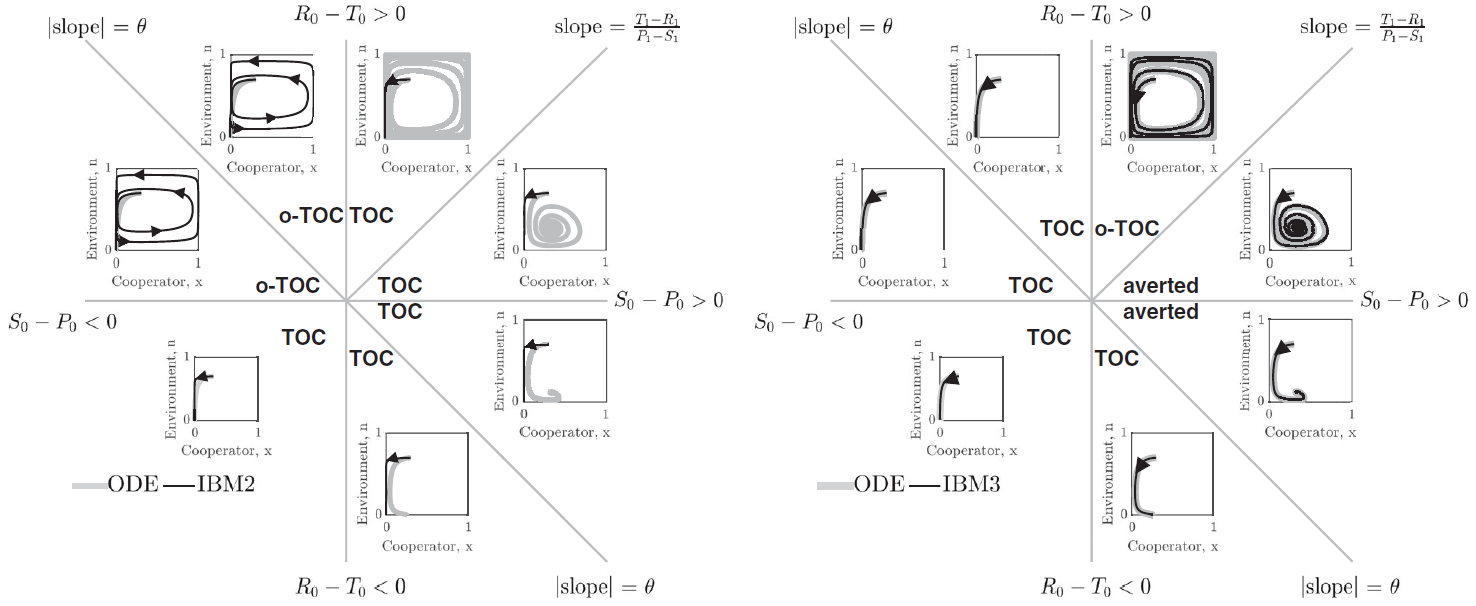
\includegraphics[width=0.9\textwidth]{pictures/Coevolutionary}
	\caption{基于IBM动态与复制器模拟的策略与资源协同进化动态。}
\end{figure}

定义扩散系数$D_n$控制相对于人口动态的资源再分配。所有情况都表现出了合作者之间的空间聚集,而在异质环境动态下($D_n=0, D_n=1$),合作者与环境资源状态间也呈现了空间聚集效应。
\begin{figure}
	\label{conevol}
	\centering
	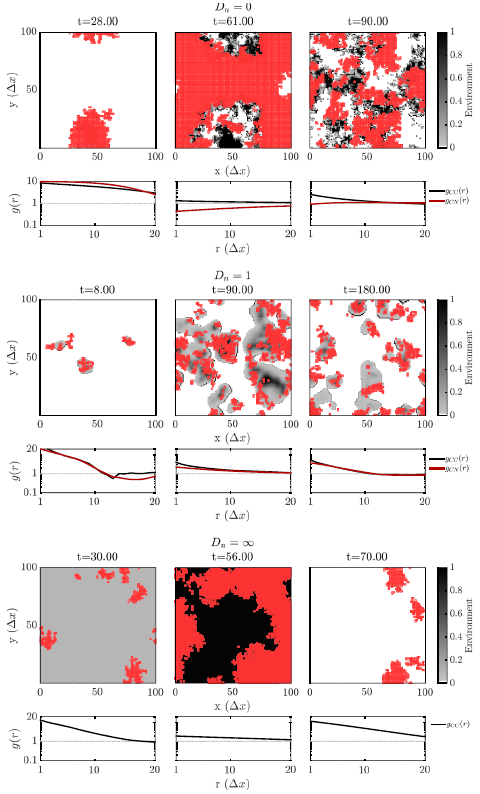
\includegraphics[width=0.7\textwidth]{pictures/D_N}
	\caption{资源与合作者的时空动态变化。背景色表示环境,红色正方形表示合作者占据的格子位置,空位被利己者占据。(顶行)$D_n=0$,合作种群的圆波向外扩散;(中排)$D_n=1$,一些小块中的合作者四处移动并分裂;(下排)$D_n=\infty$,大的合作者群体随着时间的推移而扩展和收缩,幅度逐渐增大直到全部消亡。}
\end{figure}

这一模型可进一步用来研究城市共存问题。城市是具有聚集效应的实体,它的复杂性在于它不仅是各个组分的总和,更是各个组分交互作用的产物。以城市产业格局为研究对象,则代价为动态的交易收入或支出,资源可以定义为均匀分布的人口和依赖于距离分布的企业,可结合前述思想预测在城市空间内新企业的产生。思路如下:1)收集公司经济状况及交互距离衰减情况,建立各交易的输入-输出流及当前交互矩阵;2)依赖不同的交易将公司要素进行向量化;3)建立$kN\times kN$的动态矩阵,新公司可能在有利于城市整体发展的最佳地点出现;4)在足够长的时间尺度下模拟这一过程;5)评估模拟得到的产业格局下交易的多样性和产业空间结构的适宜性。一些城市产业结构可能会导致TOC困境,即企业更追求自身利益而忽略城市整体发展。由于城市特性与多样性存在,初始状态会影响城市多样的分化。这一模拟可以帮助我们理解新兴公司在空间和规模上的分布规律。
% \chapter{空间生态系统}

% 城市的组织是复杂的。我们经常用模糊场所来描述不同空间区域在城市中所承担的分工。而一个空间位置也可能同时从属于不同的场所。城市科学的研究对象与生态系统有着类似的性质。在生态系统中,多个组分相互作用导致各自在系统中的种群密度发生变化变化。在城市中,市民对居住条件、工作条件的要求,企业对物流链、地租、工作环境的要求,也使得城市区域分化成了有一定特征的模式。在\cite{christopherson1986city}中提到了一种观点,称城市为一个工作站。这是因为城市是一个集合了各种工具,并由于其中复杂的相互依存、相互促进的关系而演化形成的生产单元。

% 这些复杂的城市元素在空间上的交互关系经过一定程度上的抽象,可以理解为城市功能在空间上涌现、迁移、或消失而组成的过程。这个过程与人类移动性\cite{molas2017field,gonzalez2008understanding,song2010limits,song2010modelling}的研究有一定的不同。城市功能的功能更具有确定性,空间特征更加明显。同时也更不可逆,是不同于基本的元人口生成模型的,也有必要单独进行建模研究。举例来说,根据\cite{banerjee2015competitive},城市标度律的形成并不一定是简单的规模效应的产物,也有可能是多方博弈的结果。以犯罪的超线性为例:默认的假设是,犯罪的超线性扩展与其他城市属性一样,是由于规模效应而产生的(也就是说,犯罪分子之间更多的联系会增加犯罪的收益)。但是,我们通常忽略的一个事实是,犯罪的发起与城市人口呈线性关系,执法人员的数量与城市人口亦呈线性关系。在\cite{banerjee2015competitive}的模型中,犯罪与执法的博弈机制成功复现了上面的标度律机制。并且该模型亦能解决某些特定类型犯罪的线性标度行为。可见,基于微观元素交互的空间模型有着比依附型生成模型更加丰富的内涵。

% 现代城市空间通常不是自然涌现的,而是经过谨慎规划的、较为规整的图案。传统经济地理研究中,对城市规整性研究主要在于定性分析\cite{colonna2002proposal}和街道生成模式\cite{barthelemy2008modeling}。路网的建模主要基于结点连接的复杂网络。而实际上,这些研究的地理基础依然有待确认。空间网络的建立隐含了路网空间和二维平面等价的假设。而在一些研究中\cite{DURRETT1994363}已经证明,并非所有的空间关系中,建立空间网络与在连续时空建模都是都是等价的。只有在确认交互性质的空间网络中,离散网络的连续化才是有意义的。

% 而在更大的尺度上,每个城市的形成是空间资源向中心集聚的过程。所以,城市之间的距离经常不是空间优化的结果。这带来的后果就是城市群自然而然的有着拓扑网络的特征。这个过程中的一些特定规模是很重要的。城市的整体意义是,大部分的沟通需求可以在一天之内完成。这给了城市功能区的组织一些客观限制\cite{schwanen2002travel,gordon1989influence}。另一方面,随着交通工具的进步,通勤速度的增加使得城市可以容纳的空间更大。更多的居住区带来的基本需求的拓展(如餐馆、公园)在空间上体现出了复杂的形态。这也可以看作是新城市聚落的形成。事实上,在生态学上有对聚落形成的理论,关注了局部生态的稳定性和可持续发展性\cite{nowak1992evolutionary}。近年来的一些新理论\cite{PhysRevLett.122.148102}表明,不同个体之间的竞争必然会导致所谓“公地悲剧”\cite{hardin1968tragedy},但合理的调控和空间纵深可以给这种现象一些缓冲。我对此的理解是,虽然复杂产业结构下的城市衰退是一定会出现的,但是这只是自组织城市体系经济周期的一个部分。这种有周期的变化比竞争性环境的确定性损失要优异的多。这也是城市设计者应该注意控制的城市结构状态。

% 本章将讨论空间演化博弈模型建立的理论基础、社会网络的结构与广义的共存与嵌套问题、以及大型系统的稳定性准则。在本章的最后,我们介绍了永续公地悲剧模型的工作。我们期望本章的工具与结论可以揭示:空间作为一个独立的维度,比网络性质有着更丰富的内涵,不能完全用点线模型进行抽象;我们也希望本章的内容可以给时间地理学一些新启示。

% \section{社会网络的层级结构与共存问题}

% 由于城市的形成是空间资源向中心集聚的过程,城市之间的距离经常不是空间优化的结果。这带来的后果就是城市群自然而然的有着拓扑网络的特征。社会网络的层次结构有着本质的空间特征。生态学中最初的层级结构就是用空间实例来描述的:岛屿上物种的类型是随着岛屿与陆地的距离而递减,因此岛屿上物种的组成是层层镶嵌的。在生物自养网络\cite{Bascompte9383}中,我们可以广泛观测到层次结构的出现。后面有一系列工作对这个现象进行了解释。比如\cite{bastolla2009architecture}说嵌套性可以减少物种之间的竞争,并且这种结构对某物种突然消亡情况下的生态系统有着鲁棒性;\cite{thebault2010stability}讲模块度(一个衡量复杂网络的module的量)和嵌套性分别产生于跨营养级和同一营养级;\cite{Allesina2012}是May于1972年工作的拓展,里面讨论了嵌套性对网络的局部稳定性是不利的;\cite{james2012disentangling}说的是nestedness就是一个伪概念,对社群结构完全没有好处;\cite{suweis2013emergence}是说用最优化的思路来看嵌套性是如何出现的;\cite{rohr2014structural}说的是嵌套性可以提高系统的结构稳定性。我们关心这个问题的原因则是为什么生态系统会出现层级结构。在地学中,层级结构可以理解为地理要素的相互依存关系。大场所圈定小场所,小场所圈定同质人口,具有哪些特征异质人口可以共同出现在同一片区域。我们知道,生态学的理论导向在于解释为什么多物种可以共存。

% 我们从两个角度讨论共存问题。分别是局部稳定性和结构稳定性。

% 局部稳定性指的是在系统稳定的状态下给系统一个小的扰动,系统恢复原状的能力。而结构稳定性则是系统的故有状态。与物种的选取有关。前者的讨论始于Robert May的一篇文章\cite{may1972will}. 改文章基于Gardner和Ashby实现的计算机模拟动力系统的结论:大型复杂系统只能在一定临界程度的连通性上面是稳定的。他们的结论是基于大小为4,7,10的系统的计算机模拟研究。May在自己的工作中通过更多的变量来完善这个研究。找到稳定与不稳定的界限仍然是研究问题的关键。本实验中,作者采用的记号有:连通率\(C\),物种数\(n\)。物种之间的关系通常是非线性的。但是这样的系统都可以在均衡点附近做泰勒展开式。系统的均衡就可以由这个方程刻画:\[\frac{dx}{dt} = Ax\]矩阵\(A\)的对角线元素设置为\(-1\),这是为了考虑进时间因素。每个元素都等概率的是正数或者是负数。然后取各种值的概率都是相等的。我们将他们的均值设置为\(0\),方差的均值设置为\(\alpha\)。方差可以作为平均交互强度的代表。随机性只在选择物种的时候出现。之后的演化过程中,系统就是完全确定的了。我们有一下结论:系统是稳定的,当且仅当\(A\)的所有特征值都有负的实部。如果\(\alpha\sqrt{n}<1\),系统几乎一定是稳定的;如果\(\alpha\sqrt{n}>1\),系统几乎一定是不稳定的。相变区域的宽度正比于\(n^{-2/3}\)。我们将系统的连通度\(C\)定义为非零元素的比例。有了这个量之后,\(\alpha^2C\)就取代了\(\alpha^2\)的角色。系统稳定的临界概率\(\alpha\sqrt{nC}\)。


% 结构稳定性的概念最早由菲尔茨奖得主Thom提出\cite{thom2018structural}。它的一个困难是估计取值过为艰难。很多时候只能靠模拟来估计。但由于生态系统的高端复杂性,这种估计方式有时会导致估计的结果的置信度过低。


% 对于生态的话题,这个采样方式有着很普适的作用。

% 12物种的群落,连通度是15\%,稳定概率为0;但是3个4物种的群落,连通概率是45\%,这样的群落有35\%的概率是稳定的。

% 四十年前,May证明了,足够大或复杂的生态网络持续存在的可能性接近零,与之前的预期相反。可以分析物种随机相互作用的大型网络。然而,在自然系统中,物种对具有明确定义的相互作用(例如捕食者
% -
% 猎物,共生或竞争)。在这里,我们将May的结果扩展到这些关系,并发现稳定的\textbf{捕食者
% -
% 猎物相互作用}与不稳定的\textbf{共生和竞争}相互作用之间存在显着差异。我们为所有案例提供分析稳定性标准。我们使用这些标准来证明,当一个现实的食物网结构被施加或者存在大量弱互动的优势时,捕食者
% -
% 猎物网络的稳定概率会降低。同样,在二分互惠网络中,稳定性受到嵌套性的负面影响。通过将网络结构和相互作用强度的贡献分离到稳定性,可以发现这些结果。只要捕食者
% - 猎物对紧密耦合,稳定的捕食者 -
% 猎物网络可以是任意大而复杂的。稳定性标准可广泛应用,因为它们适用于任何微分方程组。

% \begin{itemize}
% \item
%   May的定理:

%   \begin{itemize}
%   \item
%     交互矩阵\(M_{S\times S}.\)
%     描述了\(j\)对\(i\)在均衡点附近的影响。在他的工作中,对角线的系数是\(-1.\)
%     其余的系数以概率为\(C\)从一个确定分布中取,以概率为\(1-C\)取为\(0.\)
%     对于这样的矩阵,只要复杂度\(\sigma\sqrt{SC}>1,\)稳定的概率就是\(0.\)
%     局部稳定性衡量了一个系统经过扰动后回到均衡的概率。对于不稳定的系统,即使极小的扰动,都会使得系统远离均衡。这潜在的会使得一些物种消失。所以我们基本上不可能见到过于丰富的物种丰富度,或者过于高的连通度。数学上,一个均衡是稳定的,如果交互矩阵所有的特征值的实部都是负的。
%   \item
%     局部稳定性只是均衡点附近的性质。但是自然系统通常被认为是远离均衡的。但是,基于局部稳定性的方法还是很适合分析聚星系统。这些系统的经验的参数化通常是不适用的。这些方法是通用的,所以这些方法可以用到各种微分方程系统中。
%   \item
%     May的矩阵有着随机的结构。每一对的交互都有着随机的交互可能。但是,这种随机结构也显示,对于大的\(S\),我们可以将这种随机性翻译成确定的交互频率。所以这种矩阵可以描述交互的很精确的结构。举例来说,捕食-被捕食交互比自养交互要频繁一倍。
%   \end{itemize}
% \end{itemize}

% \section{人群交互模型}

% 这个部分主要基于几篇文章:Simplicial Models of Social Contation\cite{IacopiniSimplicial}和Spatially Distributed Social Complex Networks\cite{PhysRevX.4.011008}

% 人类局部交互模型的通常假设是短程交互和长期迁移的组合。每个个体(agent)有一定强度的个人属性,这个属性可能会被其他人影响,进而发生改变。一个例子是人类方言的变迁过程\cite{PhysRevX.7.031008,seoane2018coexistence}。

% 局部交互的方法通常由简单交互过程(基于Ising模型)或者博弈分析(基于纳什均衡)\cite{grimalda2016social,Mussa2019Urbanity} 来得到。Schelling引入了社会科学中最早的基于主体模拟的模型之一。 该模型显示,即使人们只是轻微地偏爱和同色的邻居一起生活,社会也会发生完全隔离。这个模型已经被社会科学家广泛讨论,并被物理学家使用与双相Ising模型和其他系统的类比进行了分析。\cite{Durrett14036}研究了元人口版本,该模型模拟了将城市划分为邻域的过程,并且我们对我们的知识进行了第一个分析,从而给出了有关均衡结构的详细信息以及密度的明确公式。


% \section{Rick Durrett的几个工作}

% 在这里我们希望介绍几个在地学领域较少有人关注,却十分有趣随机空间模型的工作。这些工作展示了一类基于空间演化博弈的模型在流行病学和城市生态研究方面的潜力。他总结的一些已有结果的解析方式已经在\cite{durrett2007random}中发表。

% The Importance of Being Discrete (and Spatial)\cite{DURRETT1994363}一文建立了离散的空间模型在人口动力学中成立的理论基础。四种对空间分布系统动力学进行建模的方法:平均场方法(用常微分方程描述),其中每个人都被认为具有与其他每个人互动的可能性相同;小团体模型,将离散的个人分为小团体,而无需其他空间结构;反应扩散方程,其中最小个体分布在空间中;以及交互作用的粒子系统,其中个体是离散的,并且空间被明确地表示出来。文章将这四种方法应用于空间分布种群中物种相互作用的三个示例,并比较它们的预测。每个代表关于生物学的不同假设,因此,它们之间的比较具有生物学以及建模上的含义。在第一种情况下,所有四种方法都一致,在第二种情况下,空间模型与非空间模型不同,而在第三种情况下,具有离散个体的随机模型与基于微分方程的随机模型不同。这说明了离散建模对于与粒子系统相关的极限反应扩散方程可以具有与简单地将扩散项添加到平均场方程而获得的不同的定性行为。

% 草原与树林的演化规律与工农业城市的演替有着很多相似之处\cite{durrett2018heterogeneous}。作者利用非同质空间上的Lotka-Volterra模型导出了二者可以在指数级别时间共存的事实。并且在初始转换之后,二者分异会十分明显。


% \section{社群结构的新理解}

% 近十年来,学界对生成模型的研究不仅仅限于联系的建立,更在于社会网络功能的形成。由于社群结构可以被看作城市生活的基本单元,进而划分空间集聚和空间异化效应的特征尺度,社群结构的定义与性质成为了一个很重要的研究对象。我们重点考察的有两个方面,首先是社会网络的层级结构(Hierarchy),其次是社会网络的社群形成规律。

% Hébert-Dufresne等人在2011年的文章\cite{PhysRevLett.107.158702} 中提出了结构偏好依附模型(Structural Preferential Attachment)。该模型可以生成复杂网络的很多性质。比如尺度无关性、模度性和自相似性。并且将这些性质统一在不以连边为基础的的无标度网络系统中。这带来了一个新的观测复杂网络的视角:社区(在结点和边之外的视角)。这个模型可以通过预测其社群结构来复现社会/信息网络。更重要的是,结点和社群是如何连通的。而这通常是一个自相似的结构。

% 我们首先来理解如何将空间对象抽象成网络。网络可以看作是空间对象的同质个体之间的关联模式。进而一个定义良好的网络抽象应该自然而然是无标度的,因为抽象尺度应该与问题本身是无关的。这个理念的正确性保证了\emph{采样}在复杂网络研究中的有效性。与此相关的是\cite{PhysRevLett.107.158702}中的一个重要观念:将复杂系统简化为最简单的形式,同时保留其重要属性,有助于独立于其性质对行为进行建模。我们认为,抽象出来的网络可以构建对不同是一个普适类。偏好依附(preferential attachment)就是一个重要的普适类。这个机制可以解释各个领域中富者愈富的情形。

% Some features of the spread of epidemics and information on a random graph

% 随机图是社会和技术网络的有用模型。迄今为止,该领域的大多数研究都涉及图形的几何特性。 在这里,我们关注网络上发生的过程。 我们特别感兴趣的是,它们在网络上的行为与均匀混合种群或在生态模型中常用的规则格上的行为有何不同。

% \section{公共地悲剧问题}

% 公共地悲剧(tragedy of the commons,TOC)是Garrett Hardin探索并定义的一种社会困境,它发生在两个人或群体选择不同的策略来利用有限公共资源的时候。个人出于自身利益耗尽公共资源,综合收益将劣于个体间合作、有节制地利用资源得到的利益。在宏观尺度上,TOC呈现于群体决策与环境层面,而在个体水平上,则与个体奖励机制的差异相关。由TOC困境引发的进化动力学问题可以模拟为来自两个群体(合作者和利己者)的个体频率的变化。个体间产生互动并取得收益,收益大小取决于自身及其他个体的策略,可以通过收益矩阵进行建模:
% \[A = \begin{Bmatrix}
% R &S \notag\\T &P
% \end{Bmatrix}\]
% 其中,$R$表示合作的奖励,$T$表示利己的收益,$S$表示他人放弃合作而自身选择合作后的收益,$P$表示互相背叛的惩罚。TOC困境发生的条件为$T>R>P>S$。收益表示系统的适宜度,它决定了合作者(频率为$x$)和利己者(频率为$1-x$)的数量变化,可由下式表示:
% \begin{equation}
% \dot{x} = x(1-x)[r_c(x,A)-r_D(x,A)]
% \end{equation}
% 其中,$r_c$,$r_D$分别为合作者与利己者的适宜度收益,可表示为$r_c=Rx+S(1-x)$,$r_D=Tx+P(1-x)$。

% 与标准的博弈论假设不同,TOC困境中的收益会随着反复决策过程中对公共资源的消耗而产生变化,考虑到这一动态变化,Weitz提出依赖于资源状态的回报矩阵:
% $$A(n)=A_0(1-n)+A_1(n), n\in[0,1]$$
% 即在资源状态为耗尽($A_0$)和充足($A_1$)的回报矩阵之间进行插值,环境状态的反馈将通过$n$来实现。当$n=1$时,个体更倾向于做利己的选择,当$n=0$时,个体更倾向于合作。由于考虑了资源状态,这一系统将呈现出新的非爆炸现象——永续公共地悲剧(oscillatory tragedy of the commons, o-TOC)。

% 协同博弈模型可以帮助我们从个体层面理解人口噪声和空间交互对社会环境和资源动态变化产生的影响。这一模型用平均场方法导出了合作者的极限分布,同时验证了局部交互会导致空间分异的形成。由图\ref{conevol}可以看到,o-TOC呈现出持久的收敛于边界的振荡。

% \begin{figure}
% 	\label{conevol}
% 	\centering
% 	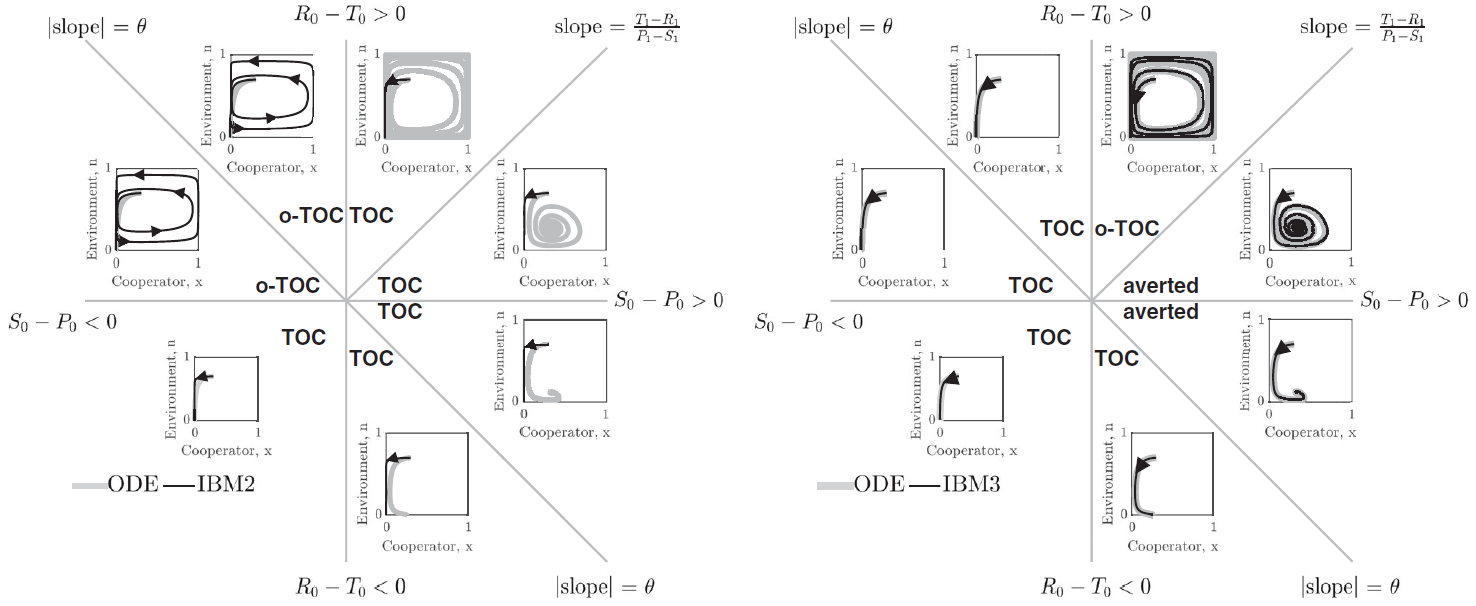
\includegraphics[width=0.9\textwidth]{pictures/Coevolutionary}
% 	\caption{基于IBM动态与复制器模拟的策略与资源协同进化动态。}
% \end{figure}

% 定义扩散系数$D_n$控制相对于人口动态的资源再分配。所有情况都表现出了合作者之间的空间聚集,而在异质环境动态下($D_n=0, D_n=1$),合作者与环境资源状态间也呈现了空间聚集效应。
% \begin{figure}
% 	\label{conevol}
% 	\centering
% 	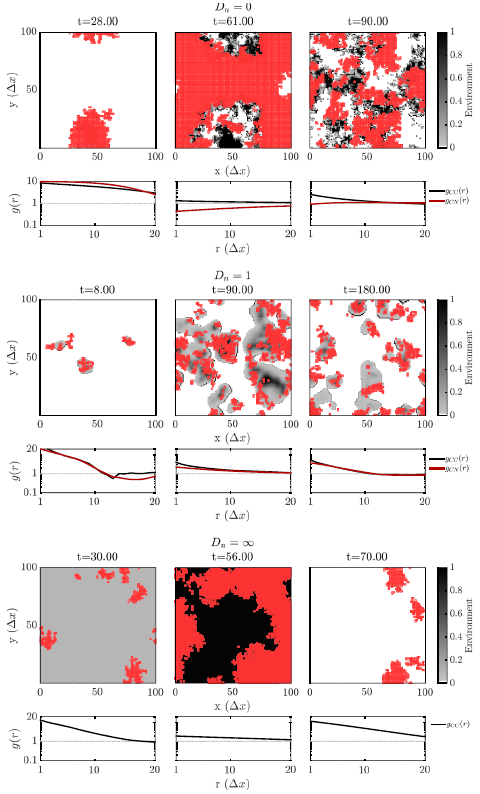
\includegraphics[width=0.9\textwidth]{pictures/D_N}
% 	\caption{资源与合作者的时空动态变化。背景色表示环境,红色正方形表示合作者占据的格子位置,空位被利己者占据。(顶行)$D_n=0$,合作种群的圆波向外扩散;(中排)$D_n=1$,一些小块中的合作者四处移动并分裂;(下排)$D_n=\infty$,大的合作者群体随着时间的推移而扩展和收缩,幅度逐渐增大直到全部消亡。}
% \end{figure}

% 这一模型可进一步用来研究城市共存问题。城市是具有聚集效应的实体,它的复杂性在于它不仅是各个组分的总和,更是各个组分交互作用的产物。以城市产业格局为研究对象,则代价为动态的交易收入或支出,资源可以定义为均匀分布的人口和依赖于距离分布的企业,可结合前述思想预测在城市空间内新企业的产生。思路如下:1)收集公司经济状况及交互距离衰减情况,建立各交易的输入-输出流及当前交互矩阵;2)依赖不同的交易将公司要素进行向量化;3)建立$kN\times kN$的动态矩阵,新公司可能在有利于城市整体发展的最佳地点出现;4)在足够长的时间尺度下模拟这一过程;5)评估模拟得到的产业格局下交易的多样性和产业空间结构的适宜性。一些城市产业结构可能会导致TOC困境,即企业更追求自身利益而忽略城市整体发展。由于城市特性与多样性存在,初始状态会影响城市多样的分化。这一模拟可以帮助我们理解新兴公司在空间和规模上的分布规律。